\documentclass[10pt]{beamer}

\usetheme{Warsaw}
%%%%%\usecolortheme{crane}
%%%%%\usecolortheme{orchid}
% \usecolortheme{orchid}
\definecolor{azul}{rgb}{.10,.20,.3}
\usecolortheme[named=azul]{structure}
\usefonttheme{structurebold}
%\usefonttheme{professionalfonts}
\useinnertheme{rounded}
\newcommand{\maggen}{\textbf{magGen}}
\usepackage[spanish]{babel}% division de silabas en spanish
\usepackage[utf8]{inputenc}
\usepackage{amsmath}
%\usepackage{amsfonts}
%\usepackage{amssymb}
%\usepackage{stmaryrd}
\usepackage{graphicx}
%\usepackage[all]{xy}

\setbeamercovered{transparent=5}

\subtitle[Generador de Evaluadores Estáticos para MAG]{Generador de Evaluadores Estáticos para MAG}
\title[Generador de Evaluadores Estáticos para MAG]{\maggen}
%\subtitle{Abstracci\'on: Acciones y Funciones}
\author{Gerardo Luis Kilmurray - Gonzalo Martín Picco}
\institute[U.N.R.C.]{
    Departamento de Computaci\'on\\
    Facultad de Ciencias Exactas, F\'isico-Qu\'imicas y Naturales\\
    Universidad Nacional de R\'io Cuarto}
% \date{Marzo de 2010}

\begin{document}

\frame{\titlepage}

\frame{
\frametitle{Temario:}
\tableofcontents
}

\section{\textquestiondown Que es magGen?}

\frame{
\frametitle{\textquestiondown Que es magGen?}
bla bla
}

\section{Marco teórico}
\subsection{Familia de Gramáticas de atributos Multiplanes (MAG)}
\subsection{Evaluador}
\subsection{Plan de evaluación}
\subsection{Secuancia de visita}

\frame{
bla bla
}

\frame{
    bla bla
}


\section{maggen}
\subsection{Diseño}



\frame{
    \begin{large}
        \frametitle{Tesis}

        \begin{block}{Tema seleccionado}
            Gram\'aticas de Atributos con Multiplanes de Evaluaci\'on (MAG)
            \footnote{WUU YANG. - http://www.cis.nctu.edu.tw/~wuuyang/./papers/magAPSEC.ps}.
        \end{block}
        \pause

        \begin{exampleblock}{Objetivo Espec\'ifico}
            \begin{center}
		\textbf{\\Generador de Evaluadores Est\'aticos de MAG.}
		\vspace{0.3cm}
	    \end{center}
        \end{exampleblock}
        \pause

        \begin{exampleblock}{Tesis Licenciatura}
            \begin{center}
		\textbf{\maggen}
		\vspace{0.3cm}
	    \end{center}
        \end{exampleblock}
    \end{large}
}

\frame{
    \begin{large}
        \frametitle{magGen}
        
        \begin{block}{Herramientas usadas}
	    \begin{itemize}
		\item C++\footnote{http://public.research.att.com/~bs/C++.html}.
		\item Boost C++ Libraries\footnote{http://www.boost.org/}.
		    \begin{itemize}
			\item Spirit Parser Framework\footnote{http://boost-spirit.com/home/}.
			\item The Boost Graph Library (BGL)\footnote{http://www.boost.org/doc/libs/release/libs/graph/}.
		    \end{itemize}
		\item GraphViz \footnote{http://www.graphviz.org/}.
	    \end{itemize}
        \end{block}
    \end{large}
}

\frame{
    \begin{large}
        \frametitle{magGen}

        \begin{block}{Proceso de generaci\'on}
	    \begin{itemize}
		\item Parsing de la MAG.
		\pause
		\item Generaci\'on de estructuras internas.
		\pause
		\item Verificaci\'on de propiedades inherentes a gram\'aticas.
		\pause
		\item Generaci\'on de grafos de DP, Down, DCG y ADP para cada regla y s\'imbolo.
		\pause
		\item Comprobaci\'on de ciclicidad sobre cada tipo de grafo.
		\pause
		\item Generaci\'on de Planes de Evaluaci\'on.
		\pause
		\item Generaci\'on de Secuencias de Visitas.
		\pause
		\item Generaci\'on de c\'odigo fuente del evaluador.
	    \end{itemize}
        \end{block}
    \end{large}
}

\frame{
    \begin{large}
        \frametitle{magGen}

        \begin{block}{Informaci\'on de input del generador}
            Especificaci\'on de una MAG.\\
	    \texttt{\begin{small}\\
	      \hspace{1cm}semantic domain\\
		\hspace{1.5cm}$<$sorts$>$\\
		\hspace{1.5cm}$<$operators$>$\\
		\hspace{1.5cm}$<$functions$>$\\
	      \vspace{0.1 cm}
	      \hspace{1cm}attributes\\
		\hspace{1.5cm}$<$attributes$>$\\
	      \vspace{0.1 cm}
	      \hspace{1cm}rules\\
		\hspace{1.5cm}$<$r0$>$\\
		  \hspace{2cm}$<$eqs$>$\\
		\hspace{1.5cm}\ldots \\
		\hspace{1.5cm}$<$rN$>$\\
		  \hspace{2cm}$<$eqs$>$\\
	    \end{small}}
        \end{block}
    \end{large}
}

\frame{
    \begin{large}
        \frametitle{magGen - Grafo DP}
	    \begin{center}
% 		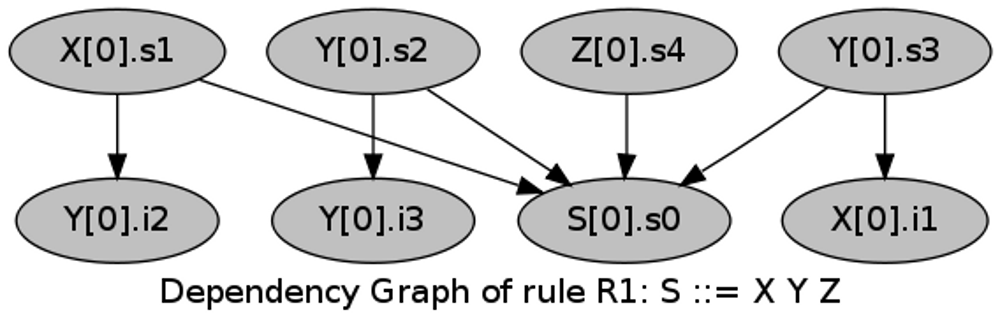
\includegraphics[scale=0.5]{./1_dp_graph.png}
		% 1_dp_graph.png: 568x188 pixel, 72dpi, 20.04x6.63 cm, bb=0 0 568 188
	    \end{center}
    \end{large}
}

\frame{
    \begin{large}
        \frametitle{magGen - Grafo Down}
	    \begin{center}
% 		\includegraphics[scale=0.6]{./6_down_graph.png}
		% 6_down_graph.png: 176x92 pixel, 72dpi, 6.21x3.25 cm, bb=0 0 176 92
	    \end{center}
    \end{large}
}

\frame{
    \begin{large}
        \frametitle{magGen - Grafo DCG}
	    \begin{center}
% 		\includegraphics[scale=0.5]{./10_dcg_graph.png}
		% 10_dcg_graph.png: 485x92 pixel, 72dpi, 17.11x3.25 cm, bb=0 0 485 92
	    \end{center}
    \end{large}
}

\frame{
    \begin{large}
        \frametitle{magGen - Grafo ADP}
	    \begin{center}
% 		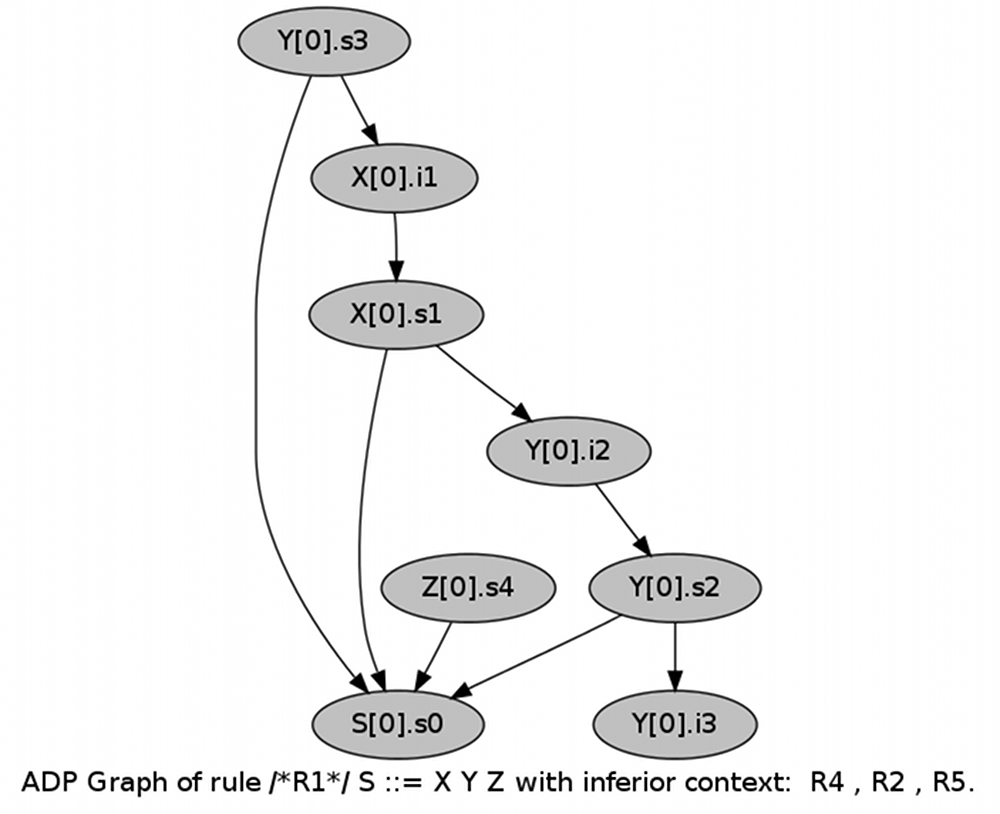
\includegraphics[scale=0.35]{./15_adp_graph.png}
		% 15_adp_graph.png: 676x572 pixel, 72dpi, 23.85x20.18 cm, bb=0 0 676 572
	    \end{center}
    \end{large}
}

\frame{
    \begin{large}
        \frametitle{magGen - Grafo ADP}
	    \begin{center}
% 		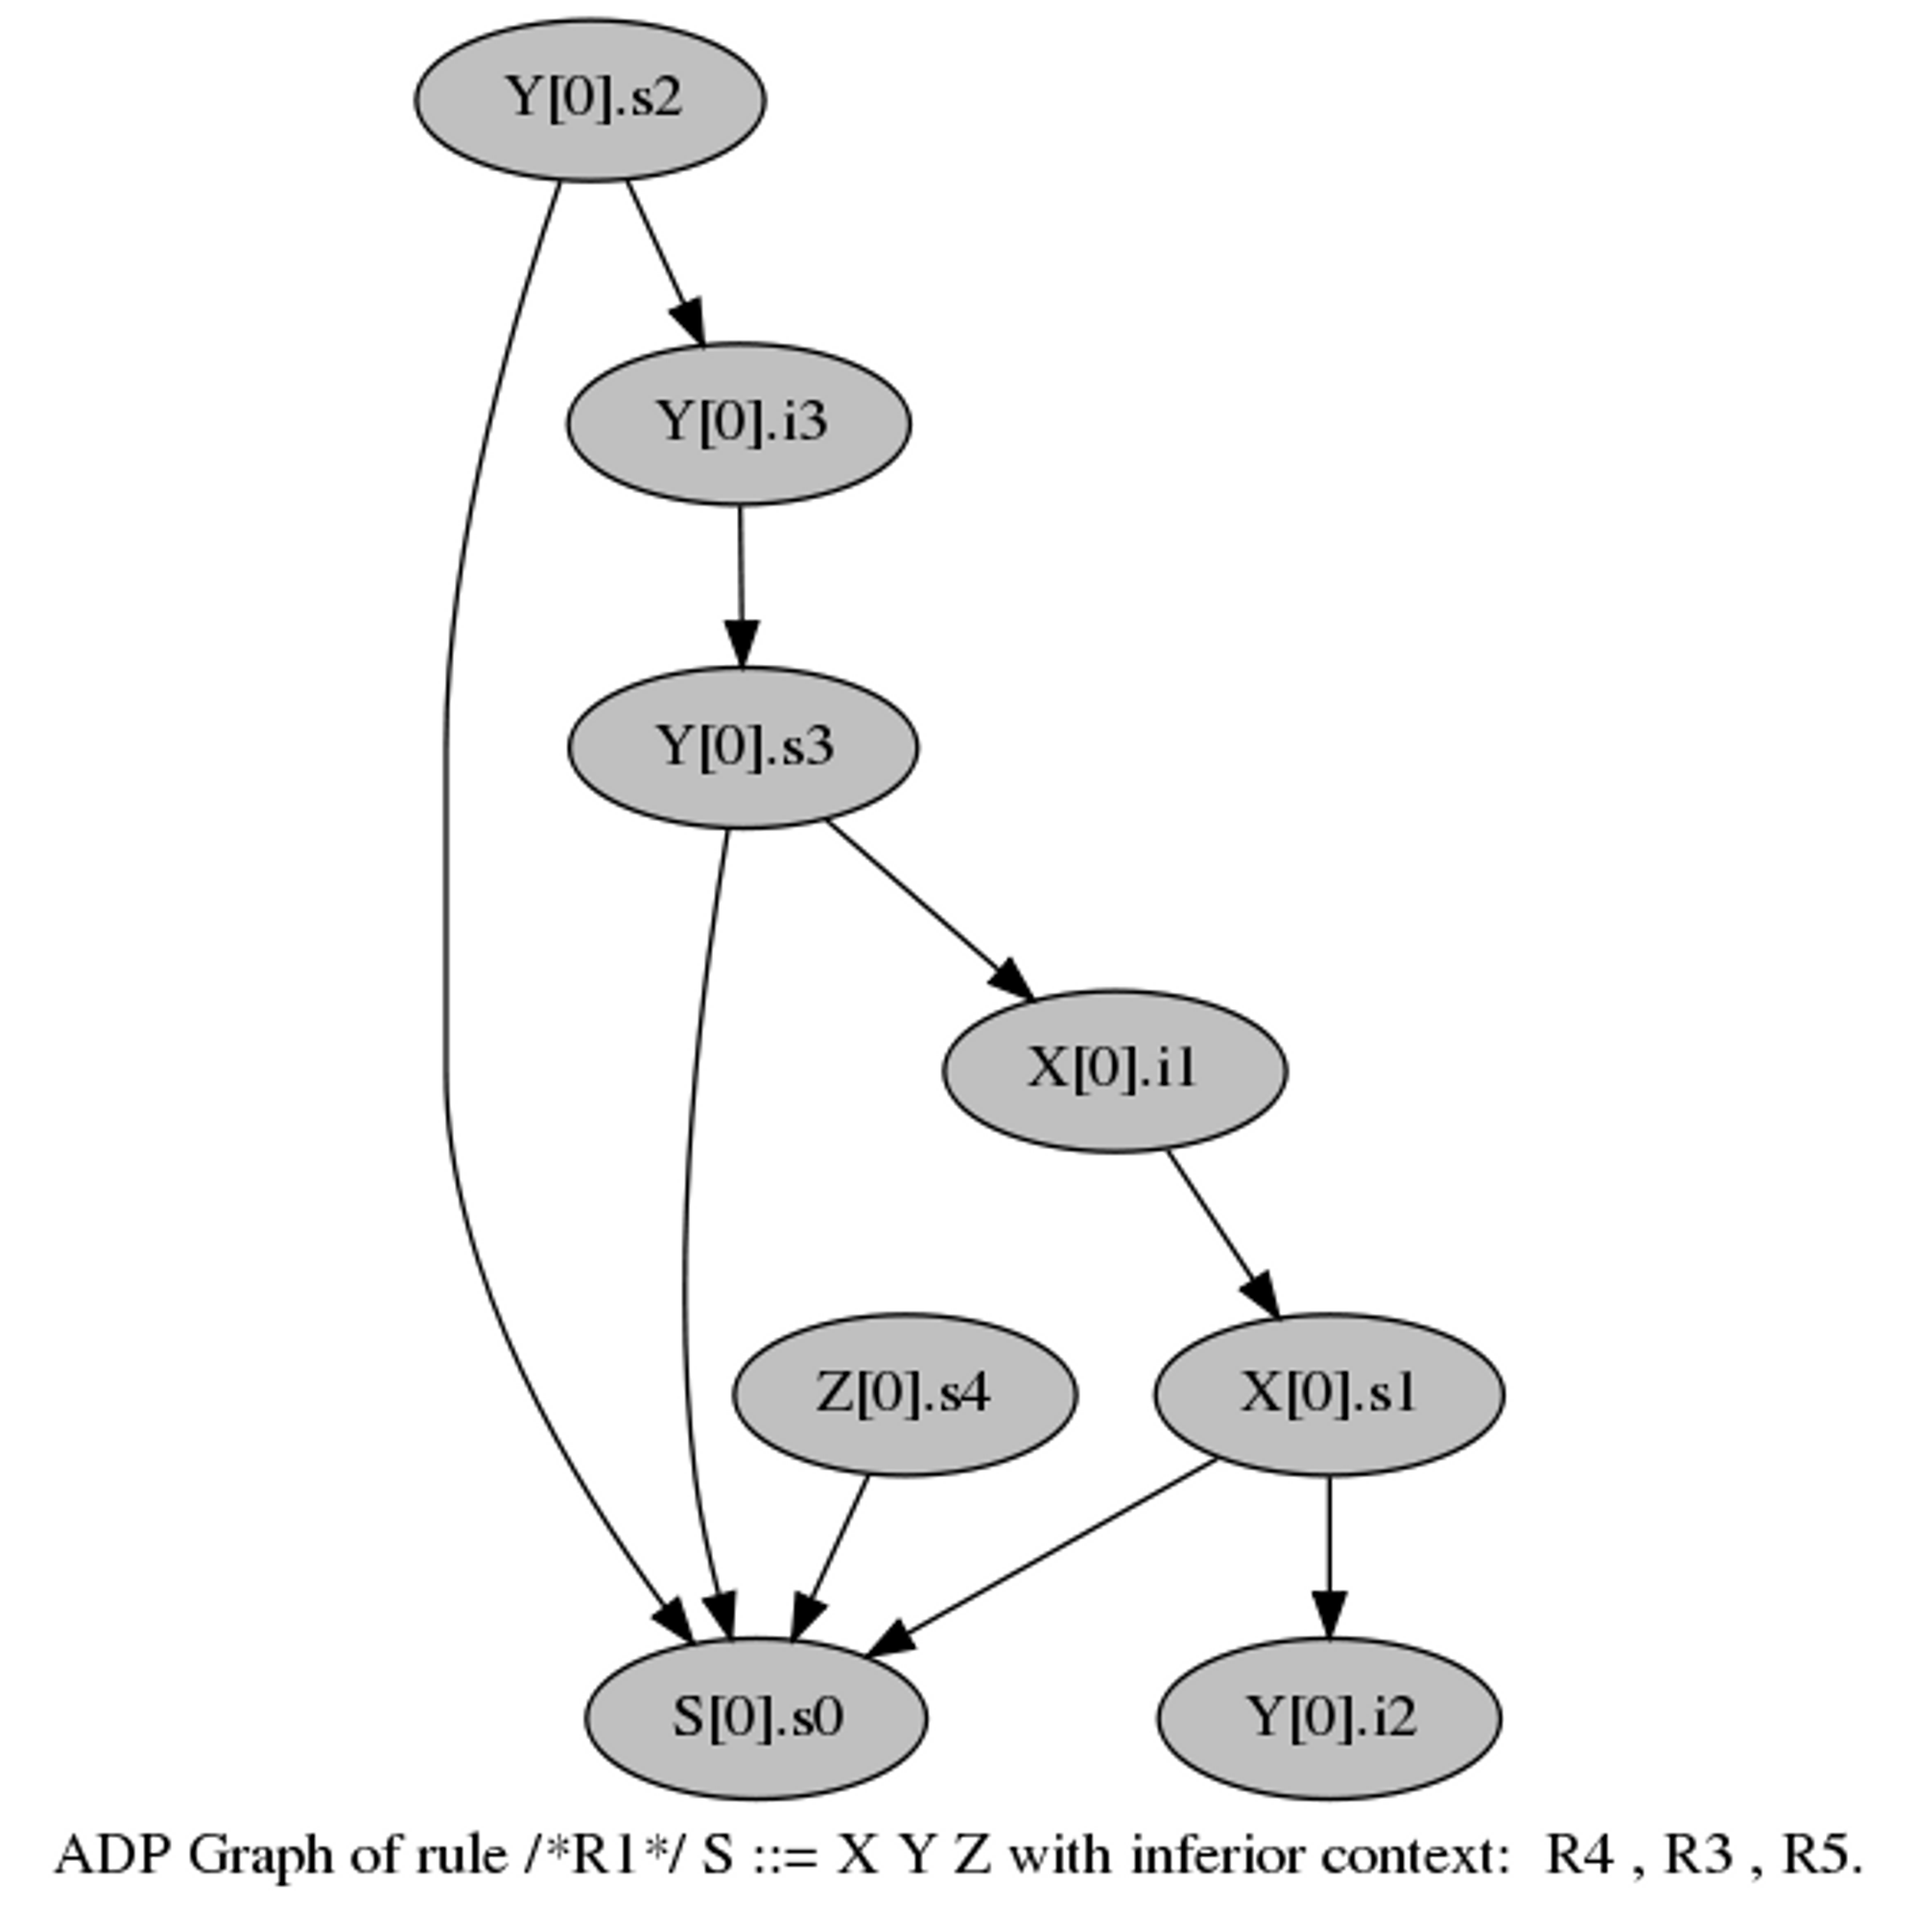
\includegraphics[scale=0.35]{./16_adp_graph.png}
		% 16_adp_graph.png: 676x572 pixel, 72dpi, 23.85x20.18 cm, bb=0 0 676 572
	    \end{center}
    \end{large}
}

\frame{
    \begin{large}
        \frametitle{magGen - Plan de evaluaci\'on}
	    \begin{center}
% 		\includegraphics[scale=0.32]{./22_plan_graph.png}
		% 22_plan_graph.png: 987x380 pixel, 72dpi, 34.82x13.41 cm, bb=0 0 987 380
	    \end{center}
    \end{large}
}

\frame{
    \begin{large}
        \frametitle{magGen - Plan de evaluaci\'on}
            \begin{center}
% 		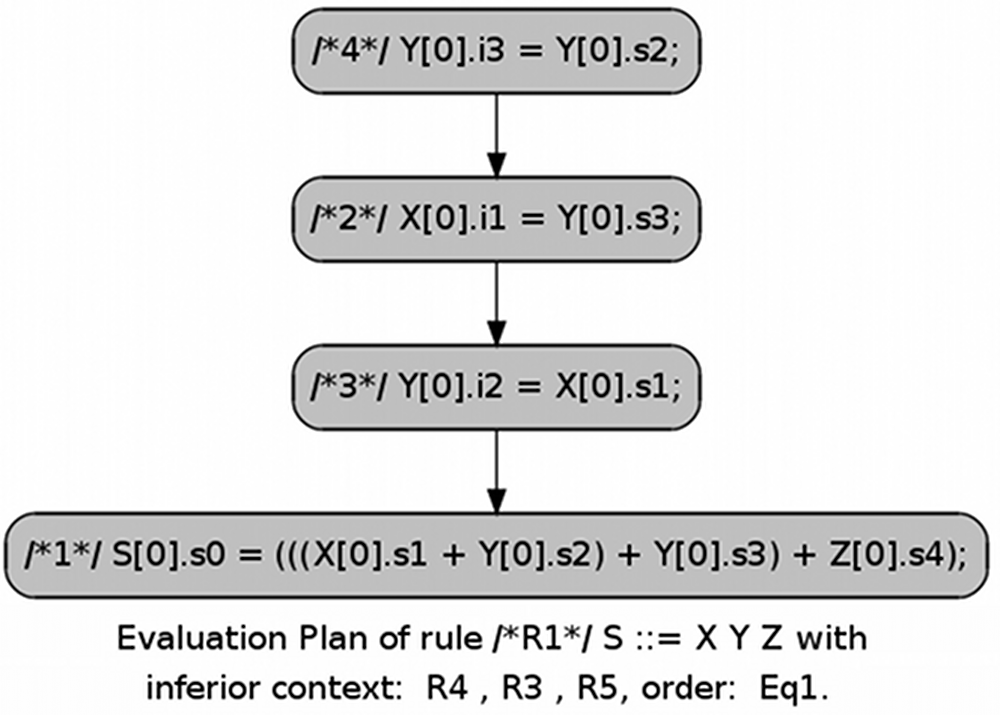
\includegraphics[scale=0.32]{./23_plan_graph.png}
		% 23_plan_graph.png: 987x380 pixel, 72dpi, 34.82x13.41 cm, bb=0 0 987 380
	    \end{center}
    \end{large}
}

\frame{
    \begin{large}
        \frametitle{magGen - Secuencia de visita}
	
        \begin{block}{Secuencia de visita generada para el plan\\ R1 $\rightarrow$ R2 R3 R4}
	    \begin{center}
		\vspace{0.1cm}
		\textbf{Visit R2 $\Rightarrow$\\
			\vspace{0.1cm}
			Compute X[0].i1 $\Rightarrow$\\
			\vspace{0.1cm}
			Visit R4 $\Rightarrow$\\
			\vspace{0.1cm}
			Compute Y[0].i2 $\Rightarrow$\\
			\vspace{0.1cm}
			Visit R2 $\Rightarrow$\\
			\vspace{0.1cm}
			Compute Y[0].i3 $\Rightarrow$\\
			\vspace{0.1cm}
			Visit R5 $\Rightarrow$\\
			\vspace{0.1cm}
			Compute S[0].s1} 
	    \end{center}
	\end{block}
    \end{large}
}

\frame{
    \begin{large}
        \frametitle{magGen}

        \begin{block}{Informaci\'on de input del evaluador}
            \'Arboles Atribu\'idos representados con AST\footnote{Attribute Syntax Tree}.
        \end{block}
        \pause

        \begin{block}{Informaci\'on de output del evaluador}
            El AST decorado\footnote{Cada uno de sus atributos se encuentran calculados}.
        \end{block}
    \end{large}
}

\frame{
    \begin{large}
        \frametitle{magGen}

        \begin{block}{Objetivo Subyacente}
            Implementar Lenguages de Prop\'ositos Espec\'ificos para problemas puntuales.
        \end{block}
    \end{large}
}

\subsection{Detalles de implementación}

\section{Comentarios Finales}

\frame {
bla bla
}

\frame {
bla bla
}

\end{document}

